
%This thesis addresses that OLAP over large property graph is important but current graph databases process graph OLAP in an overwelmingly inefficient manner, and provides an end-to-end efficient solution for it.

Being a flexible and semantic rich model for graph structured data, the property graph model has been widely adopted and we have seen emerging Graph database systems supporting this model, like Neo4j \cite{DBLP:conf/oopsla/Webber12}, PGX \cite{DBLP:conf/sc/HongDMLVC15}. Supporting OLAP (On-Line Analytic Processing) is one critical feature of modern database systems, because efficient OLAP processing is fundamental to many decision-making applications, e.g., smart business~\cite{Petermann:2014:GDI:2733004.2733034}, market analysis~\cite{DBLP:journals/corr/LamSG16}, trend monitoring~\cite{DBLP:journals/tii/FangXZAPYL14}, risk management~\cite{DBLP:journals/tcyb/ChoiCY17}. However, empirical studies show that existing graph database systems do not efficiently support OLAP workloads, especially structure wise aggregation queries. Moreover, current graph database systems do not support view-based query or materialize some ``hot'' intermediate results to serve future queries. Therefore, in this thesis, we study the efficient processing of OLAP queries over property graph data using a materialization approach.


%----------------------------------------------------------------------
\section{Property Graph Model}
\label{s:1}
%----------------------------------------------------------------------

We are living in an age with exponential growth of data, and a world that is more and more connected.  With the fast development of Web2.0 and Internet of Things(IoT)~\cite{DBLP:journals/cacm/X17f}, numerous connections of various kinds are being created every second, producing massive amount of graph structure data in the meanwhile. For example, the moment a user creates a new post on a online forum, not only a post is created,  a ``\emph{creates}'' connection between the user and the post is established as well; when a user tags a post, a ``\emph{hasTag}'' connection is created between certain tag string and the post; or in a banking scenario, when a transfer happens, a ``\emph{transfers}'' connection between two accounts is created.

To capture the rich semantic of connected real-world entities, property graph model~\cite{} is becoming more and more popular considering its flexibility for semi-structured graph data. A property graph consists of nodes, edges, and properties. Like general graph data models, nodes represent entities and edges represent relationships. Graph nodes and edges can have any number of properties, or attributes, of any type. For example, Figure \ref{fig:1} shows a simple property graph of an online Q\&A forum named www.StackExchange.com. It shows the connections among users (represented by red nodes) and posts (represented by blue nodes). Each arc pointing from a user node  to a post node represents a ``User\_onws\_Post'' connection. From the graph, we can clearly see that  there is one user who has created one post while the other usr has created 2 posts. In addition, as shown in the example, a User node can have properties like the user’s Age, Views, UpVotes and etc. (listed at the end of the picture).
%Notice that there is no restriction on what properties a User node can have.
For clear presentation purpose, we shall use a property graph dataset obtained from \url{www.StackExchange.com} through this thesis. We name this graph ``StackExchange graph''.


\begin{figure*}
\centering
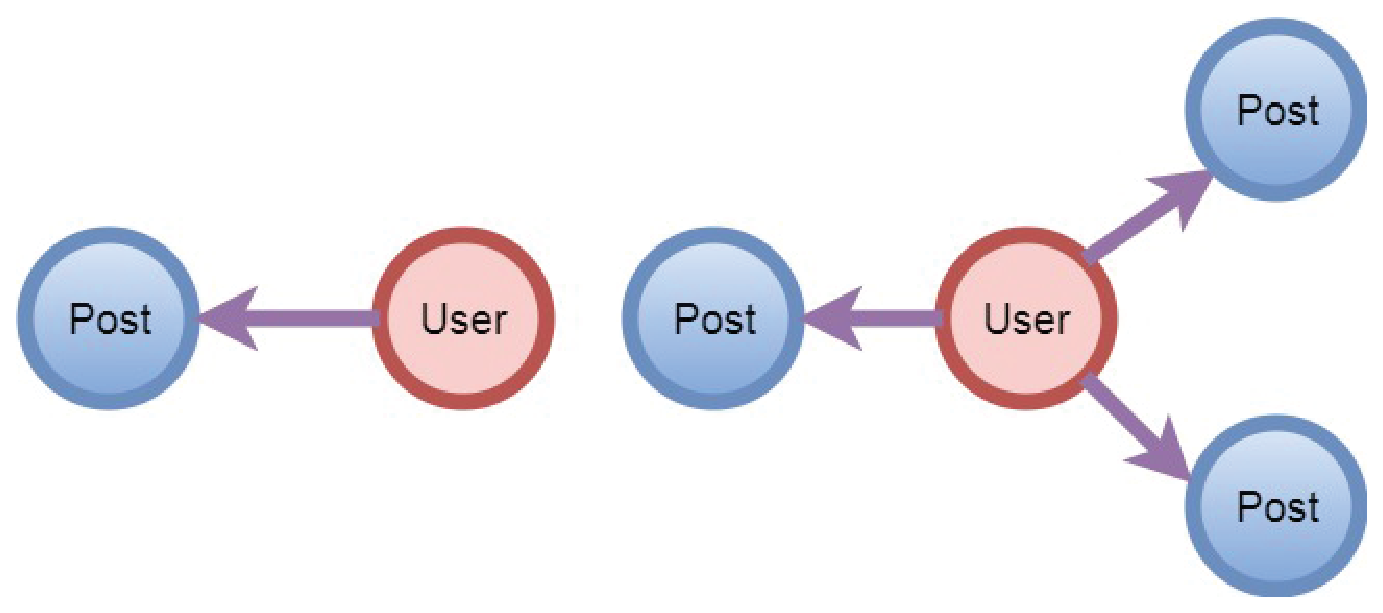
\includegraphics[scale=0.4]{pic/11.eps}
\caption{A simple property graph modeling ``users post posts''(data graph).}
\label{fig:1}
\end{figure*}


%Besides nodes and edges, in property graph nodes and edges can have any number and type of properties.


%For instance, in the exampling property graph,   That is, any node or edge could be freely attributed with any type of property. This makes a property graph very flexible in terms of property attribution.

%Property graph is an informative model as it contains not only nodes and edges, but properties of each individual node and edge as well.

Note that although the property graph model does not enforce any restriction on what properties a node or edge can have, a highlevel abstraction describing the property relations, named the meta graph, is ofen defined in practice. Meta graph demonstrates the information of entities and entity correlations on a schema level, while data graph refers to the actual graph populated from the meta graph. Figure \ref{fig:2} and Figure \ref{fig:3} are the meta graph and a snapshot of the StackExchange graph, respectively. As shown in Figure \ref{fig:2}, there are three types of entities: User (in red), Post (in blue), and Tag (in green). Each user has a property named ``View'', each post has a property named ``Score'', and a property ``Tagname'' associated with each tag. There are two types of edges being  defined: User\_owns\_Post and Post\_hasTag\_Tag.


\begin{figure*}
\centering
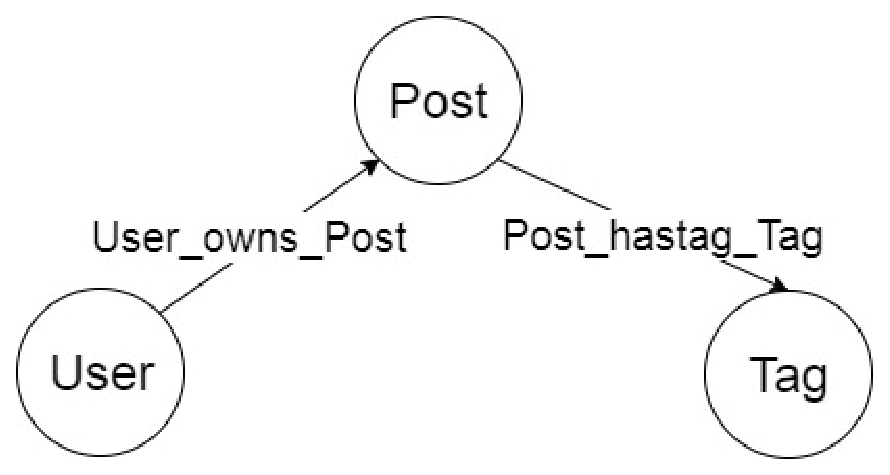
\includegraphics[scale=0.5]{pic/12.eps}
\caption{Meta graph containing User, Post and Tag.}
\end{figure*}

\begin{figure*}
\centering
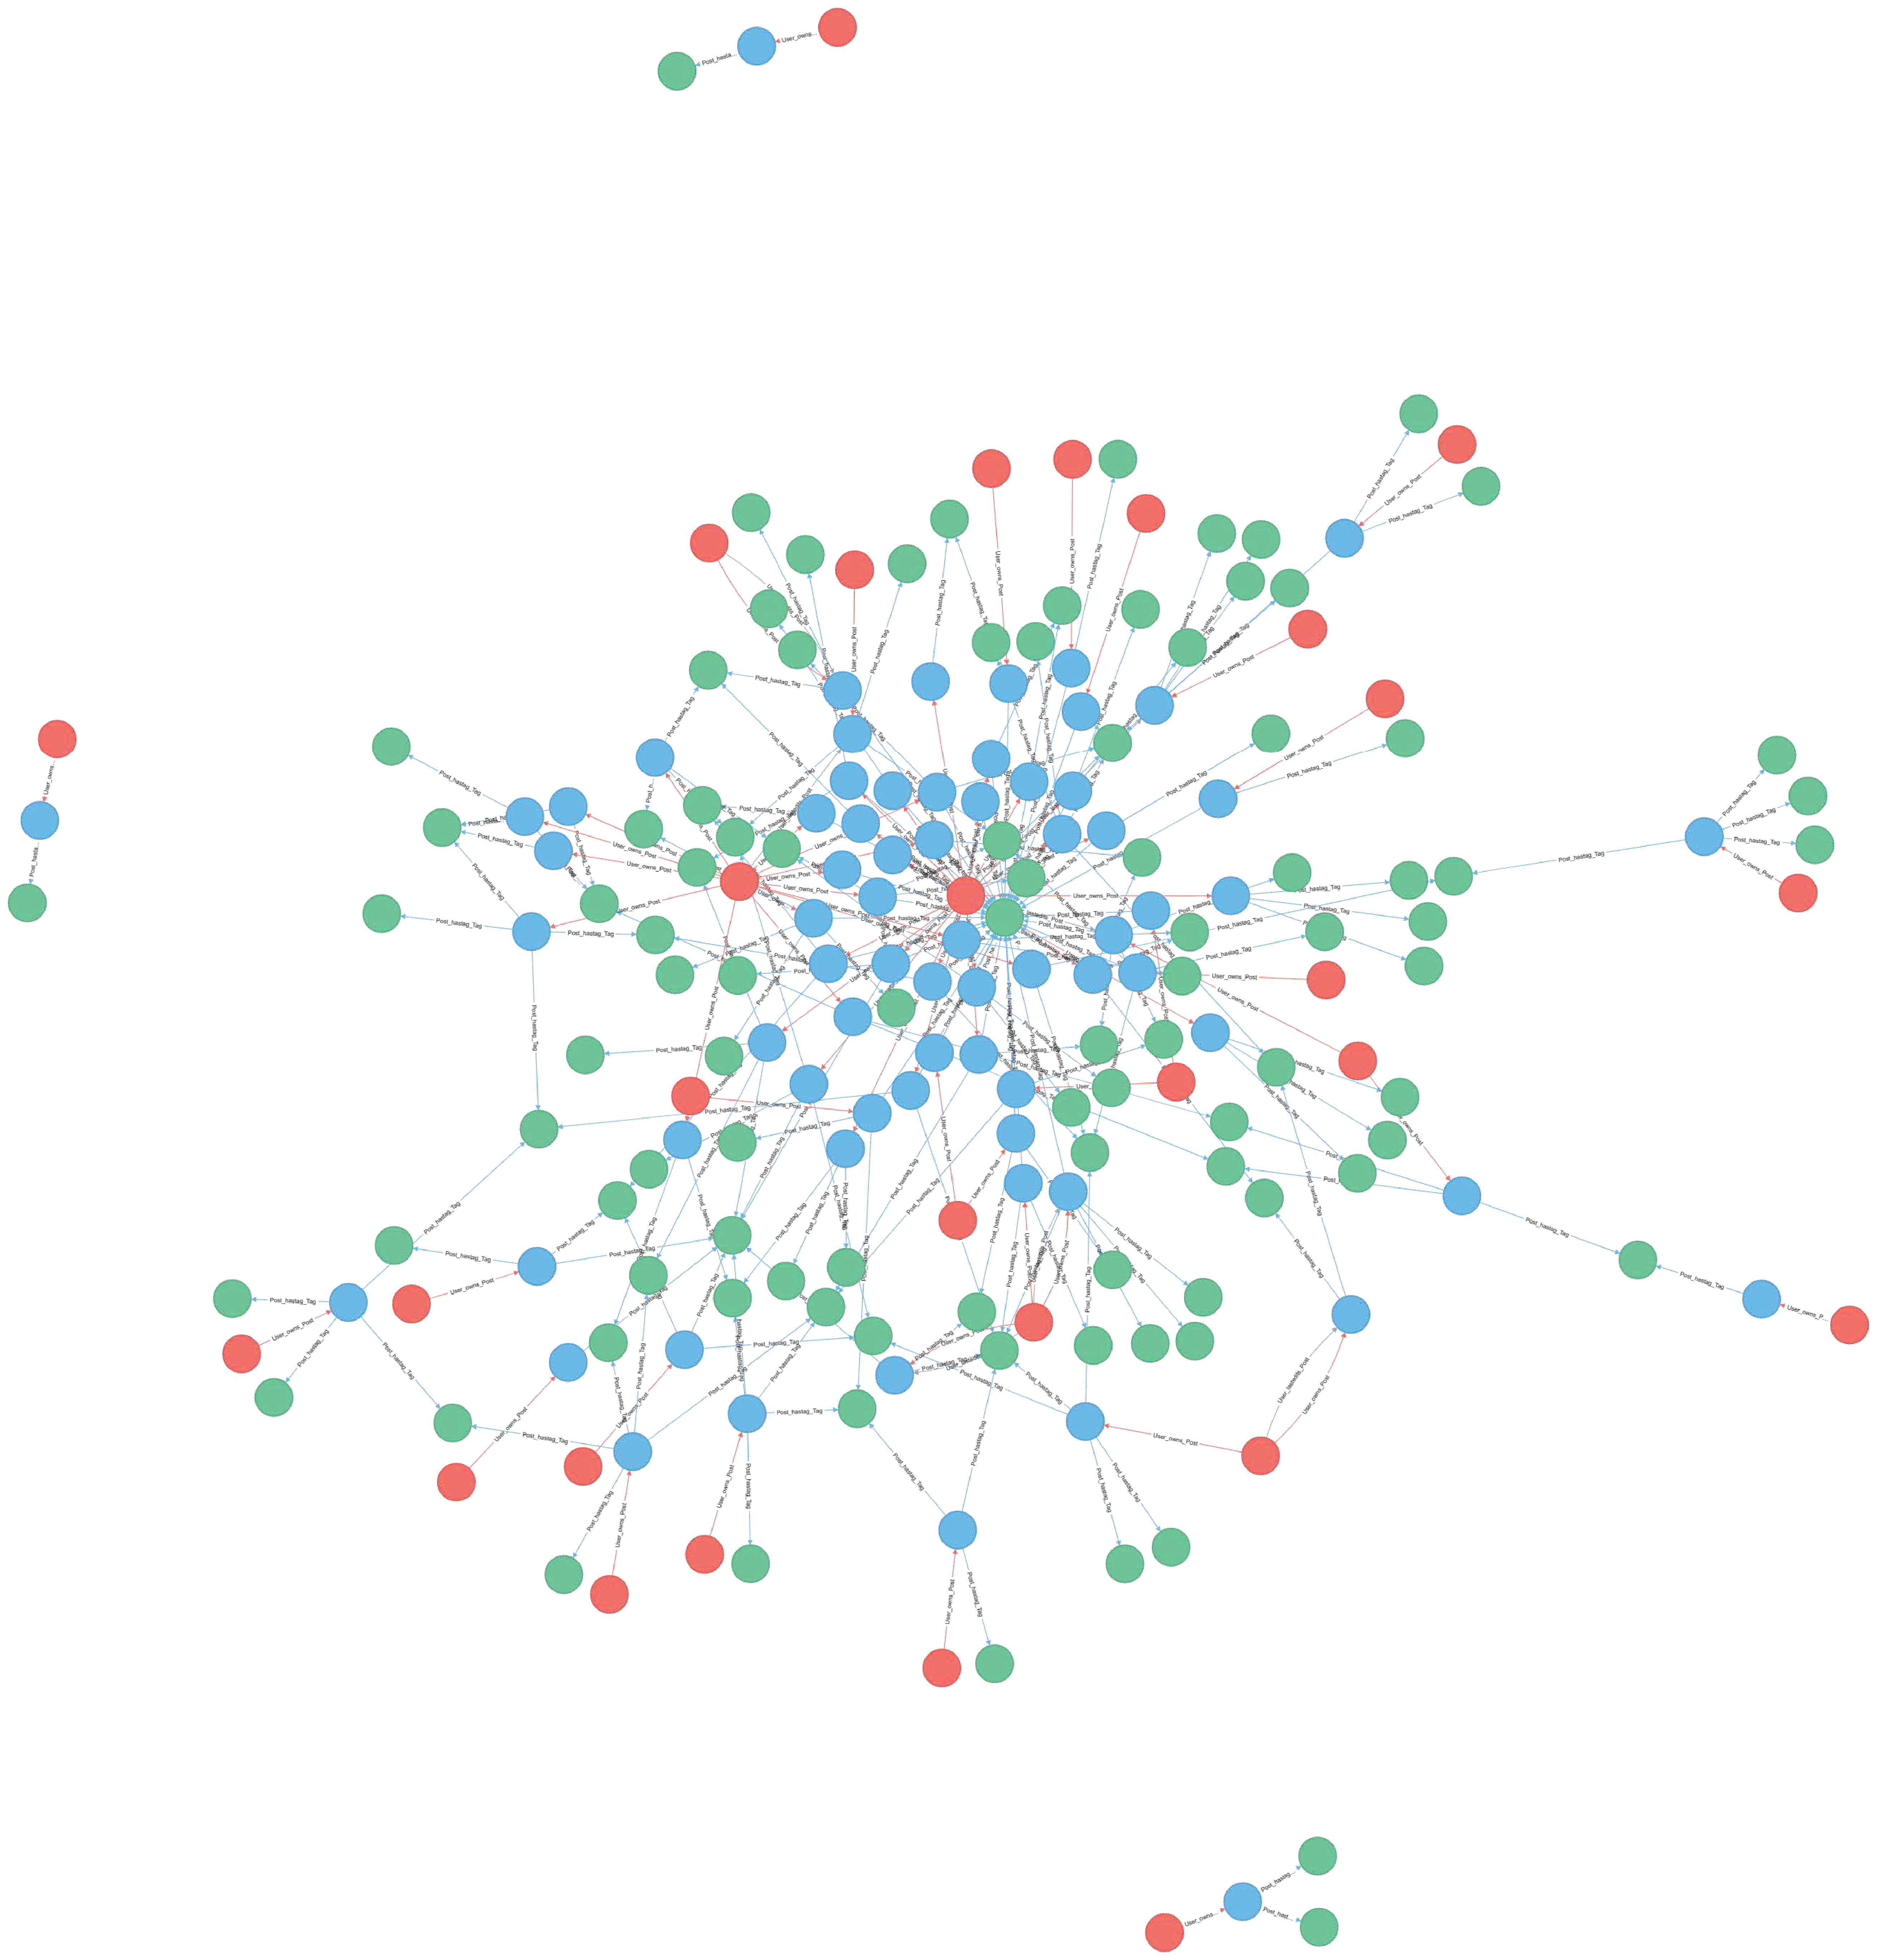
\includegraphics[scale=0.1]{pic/3.eps}
\caption{A snapshot of data graph containing User, Post and Tag.}
\end{figure*}

%----------------------------------------------------------------------
\section{OLAP over Property Graph}
%----------------------------------------------------------------------
%Among various kinds of queries, OLAP (Online analytical processing) queries play an important role in data analysis.
%\intodo{Add a few sentences to describe OLAP queries of the traditional database and warehousing applications. Showing it is important and we say performing OLAP on property graph is desired. }

In tradition databases and ware-housing, OLAP queries enable users to interactively perform aggregations on underlying data from different perspectives(combinations  of dimensions). There are three typical operations in OLAP. Roll-up operation allows user to view data in more details while drill-down operation does the opposite way. Slicing enables filtering on data. For instance, we can perform OLAP to analyze earning performance of an international company by different branch. We can perform drill-down operation by adding season as a dimension besides branch to take a closer look at profit performance of different branches in different seasons. In this case, OLAP serves as a tool for managers to better understand earning performance.

Supporting efficient OLAP processing on property graphs grants users the power to perform insightful analysis over structured graph data. For example, on the StackExchange graph, users can study the correlation between the number of UpVotes and a post's score by using the following query:

\fbox{\emph{Get the average post score grouped by user’s upvotes.} }

 If the result shows a tight correlation, it suggests that an author’s upvotes can be used to estimate the quality of his or her post when a post is freshly posted and score of the post has not been settled.


Consider another example, using a property graph dataset on music industry,  one can issue the following query to evaluate a company's strategy to increase the share of young people's market.

\fbox{
\begin{minipage}{35em}
\emph{Get the total sum of music purchases by buyers at age 18-25 grouped by music company and month}
\end{minipage}
}


For simplicity, we call such kind of OLAP query workloads over property graphs as ``Graph OLAP''. As a matter of fact, graph OLAP has already been applied in various senerios like business analysis and decision making and it is attracting increasing research interests in the database community.



%----------------------------------------------------------------------
\section{Challenges of Graph OLAP}
%----------------------------------------------------------------------

%We know that Graph OLAP is important. However there are many challenges on this topic. One of the most challenging part is efficiency issue.
%\intodo{Here you should start with a paragraph saying "Supporing efficient OLAP is traditional RDBMS or warehousing applications is a well studied topic. There are abundent literature attacking this problem from virous different perspectives, e.g. data partition~\cite{}, view selection~\cite{}, partial materialization~\cite{}, .... However, there is very few research effort on the Graph OLAP. Existing literatures concerning OLAP workload over graph data either target on accelerating graph OLAP over a special subset of property graphs~\cite{}, or focus on generic highlevel topics, such as ... \cite{},  other than time efficiency issue of query processing."}

Supporting efficient OLAP in traditional RDBMS or warehousing applications is a well studied topic. There are abundent literature attacking this problem from virous different perspectives, e.g. data partition~\cite{DBLP:conf/ismis/CuzzocreaL12}, view selection~\cite{DBLP:books/igi/Taniar10/LawrenceR10}, partial materialization~\cite{DBLP:journals/kais/DrzadzewskiT16}. However, there is very few research effort on the Graph OLAP. Existing literatures concerning OLAP workload over graph data either target on accelerating graph OLAP over a special subset of property graphs~\cite{DBLP:conf/sigmod/ZhaoLXH11}, or focus on generic highlevel topics, such as \cite{DBLP:conf/esws/MaaliCD15} \cite{DBLP:conf/icdm/ChenYZHY08},  other than time efficiency issue of query processing.

%From an academic point of view, most of OLAP studies reside in traditional relational data models, whereas studies on efficient graph OLAP are not enough. What's worse, current graph OLAP researches either

Our empirical studis show that existing graph databases do not provide efficent support for graph OLAP, especially when the graph size scales to real-word practices, which usually contains over millions of nodes and edges. %Graph databases are databases that specialize in storage and processing of property graphs. However current graph databases are not satisfactory in terms of OLAP processing efficiency over large property graphs(often with more than millions of nodes and edges).
To elaborate, Neo4j, a state-of-art graph database, processes OLAP queries in a rather straightforward manner: computing everything from scratch for each query without being aware of any history workloads. In an extreme case, even if we executed the same query repeatly with only minor change on value constraints, e.g., change the constraint of user's age from 20 to 22, the execution plan always stays the same and yields no execution time improvement.

\begin{figure*}
\centering
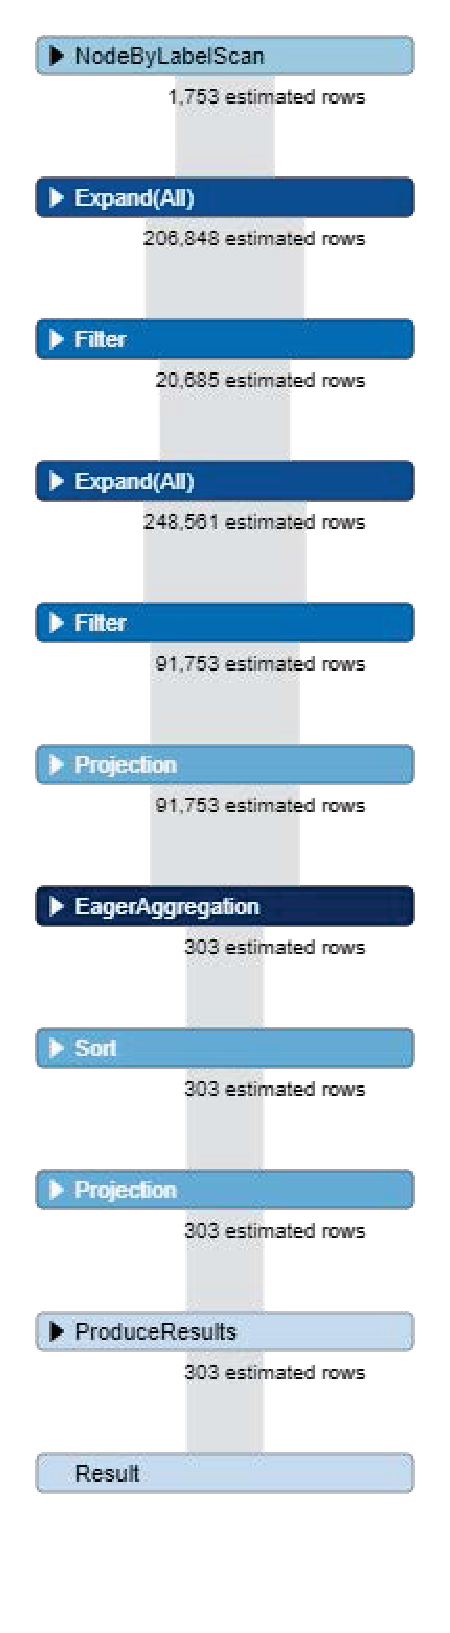
\includegraphics[scale=0.4]{pic/5.eps}
%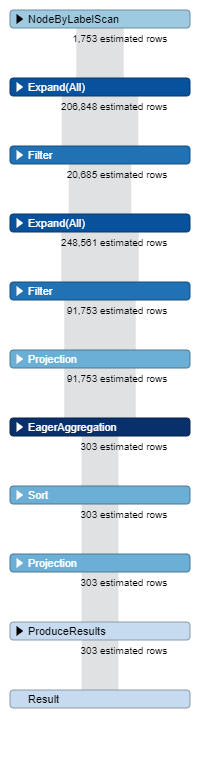
\includegraphics[scale=0.4]{pic/5.png}
\caption{Execution plans of Query \#3 for first time and fifth time.}

\end{figure*}

%This naive feature of always executing queries regardless of previous queries misses valuable information contained in previous workloads.
Valuable information extracted from history workload can be helpful to accelerate in-coming query processing. For example, the above exampling OLAP query on StackExchange graph dataset (of roughly 45GB in size) takes Neo4j more than 2 hours to process. It is frustrating for users to wait that long for the result of one single OLAP query, as it undermines interactivity which is one of the most distinctive features of OLAP. %Therefore we want to accelerate OLAP processing over large property graphs
%\intodo{Now you should explain what you can learn from previous workloads, and how these knowledge can help you with future workloads.}

As a matter of fact, history workloads provide useful information for future workloads. This is because in real case users do not generate OLAP queries randomly. Instead users often tend to be interested in some specific ``hot'' structures on a meta graph level and some ``hot'' properties. Such interest is contained in history workload and can serve as an insightful hint on future workloads. Suppose we sacrifice some memory space and materialize ``hot'' structures and properties even before future queries arrive, future queries can be faster processed.

%\intodo{Then, you need a paragraph that describe the actual challenge. Because so far you only mentioned that using something from history workload is helpful, then the problem is how to extract these information, how to decide which information should be materialized espeically when there is a space constraint.}

We know that materializing user's interested structures and properties benefits future workload processing, at the cost of extra space overhead. The real challenge is how to design a score function to evaluate the trade-off  between such benefit and cost so that we can use the score function to select best materialization. Here best materialization refers to the case where we achieve best future workload acceleration with a given memory constraint for materialization.

%\begin{center}
%	\begin{tabular}{ | l | l | }
%		\hline
%		Query 	& Time	\\ \hline
%		Query \#1	& \\ \hline
%		Query \#2	& \\ \hline
%		Query \#3	& \\ \hline
%	\end{tabular}
%	\end {center}
	
	


%----------------------------------------------------------------------
\section{Our Solution and Contributions}
%----------------------------------------------------------------------
To address the challenges discussed above, we propose a end-to-end solution for graph database to  support efficient  OLAP over large property graphs.

The essence of our solution is to precompute and materialize popular intermediate results that can be reused by future workloads. Intuitively, in real practice, most OLAP queries from the same client   tend to reside in several particular structures and properties (usually closely related with the topics that the client is interested in). Within a specific period of time, there are ``hot'' structures that the client tends to repeatedly investigate from different dimensions. Therefore, previous queries can be used as a good reference to discover structures and properties in which the client is particularly interested.

%For instance, suppose a client just executed the exampling four queries, here is what we can learn from these four previous workload:

%Structure-wise: (User)-[creates]-$>$(Post) is frequently queried. We can tell that client is interested in how users create posts. Thus it is reasonable to guess that the user is likely to issue OLAP queries involving (User)-[creates]-$>$(Post) in following queries.

%Property-wise: User.UpVotes, Post.Score, User.Age, Tag.TagName etc. More specifically, \{User.UpVotes, Post.Score\} and \{User.Age, Tag.TagName\} are frequent combinations. Thus it makes sense to guess that these property combinations are likely to appear together in future queries.

%Intuitively, if we smartly select frequently queried structures and properties based on previous workload and materialize them, they might be covered in future queries and thus be used to accelerate processing.

A good analogy of this is establishment of materialized views in relational databases and processing queries directly on materialized views. In relational databases, we are allowed to build materialized views on structures and attributes that we are interested in. Hopefully when future queries come, we can faster process them using pre-materialized views. Unfortunately, current graph databases do not support similar operations.

%Therefore we propose a system that realizes automatic and smart pre-computing and materialization based on history workload, and utilize the materialized result to accelerate future query processing.

There are two most important problems that we need to solve. One key issue is smart selection of ``materialized views''. We need to select and pre-compute those that are most beneficial for future queries. Another key issue is how to optimize a better execution plan for answering a future query efficiently using the precomputed materials.
%\intodo{here you need to use a paragraph to explain how you select materialized views, e.g., you develop a cost function. Plus, you have a scheduling policy to execute subqueries in the most time efficient way. This part is particularly important, because reader need to briefly understand you overall solution from a high level perspective.}
To address the first issue, we develop a score function to evaluate cost–performance ratio of a materialization. We propose a greedy  algorithm to  select candidate  based on their score (calculated from score function), one by one until memory limit is hit. For the second challenge, if a future query result can be directly produced using a materialization we simply do it. For other cases, we propose a scheduling policy to decompose a future query into substructures and join such substructures to produce final result.

To highlight, we summurize our contributions in this thesis as follows:
\begin{itemize}
\item {We designed an end-to-end system that realizes structure-aware OLAP query processing on graph databases using precomputation based on previous workloads.}

\item We implemented our system on Neo4j.

\item We proposed our algorithm for smart selection of structures and cuboids to be precomputed.

\item We suggested different ways for future query processing. We tested their performances and gave explanations on the performance differences.

 \end{itemize}

The following contents are organized as follows:
 we discuss the preliminaries and related work in Chapter 2. Followed by the background knowledge about  OLAP, graph databases, and Neo4j, we give a summarization of existing literatures concerning OLAP queries over graph data. In Chapter 3 we explain our solution framework and system design in details. We present the experiment design and result disucssion in Chapter 4. Chapter 5 concludes this thesis with highlight on opening questions and future work.

